\documentclass[a4paper,11pt,dvipdfmx]{ujarticle}
% パッケージ
\usepackage{graphicx}
\usepackage{url}
% レイアウト指定を記述したファイルの読み込み
\input{layout}

% タイトルと氏名を変更せよ.

\title{日本におけるデジタル化の状況}
\author{G584012025 松原 由未子}

\begin{document}

\maketitle %ここにタイトルが入る

\section{ブロードバンドの整備状況}
OECDによるブロードバンドの回数の普通に関する調査\cite{oecd}
によると、図1に示すように、日本におけてる100人あたりの光ファイバー回数の加入者数は29.0で、韓国、スエーデン、ノルウェーに続いておいて第4位になっている。

\begin{figure}[htbp]
    \centering
    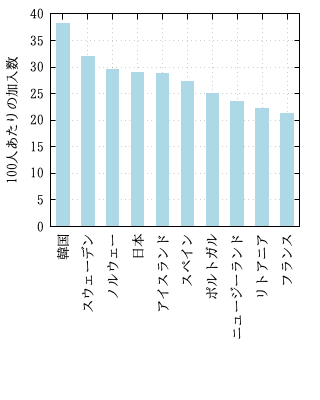
\includegraphics{fig11.png}
    \caption{光ファイバー回線の加入者数(100人あたり)}
\end{figure}

\section{デジタル競争力ランキング}
国際経営開発研究所(IMD)の調査\cite{imd}
によると、日本のデジタル競争力のランキングは表1に示すよ
うに、調査対象の64カ国中、総合で28位、技術分野で30位となっている。

\begin{table}[htbp]
    \centering
    \caption{デジタル競争力ランキング(64カ国中)}
    \begin{tabular}{|c|c|c|}
        \hline
        国 & 総合 & 技術 \\
        \hline
        米国 & 1位 & 4位 \\
        \hline
        香港 & 2位 & 10位 \\
        \hline
        スエーデン & 3位 & 8位 \\
        \hline
        デンマーク & 5位 & 3位 \\
        \hline
        シンガポール & 5位 & 3位 \\
        \hline
        \hline
        韓国 & 12位 & 13位 \\
        \hline
        中国 & 15位 & 20位 \\
        \hline
        \hline
        日本 & 28位 & 30位 \\
        \hline
    \end{tabular}
\end{table}

\section{考察}
\begin{itemize}
    \item 韓国は図1によると光のファイバーをいっぱい使われている
    \item 表1では日本デジタル競争力とても低い理由は大学教育における情報工学が少ない
    \item 表1では香港が上位にいる理由は政府が力を入れているからかもしれない
\end{itemize}


% ここから本文
% 節見出し: \section{}
% を使う

% 本文(1)
%  参考文献の参照: \cite{}
%  図番号の参照: \ref{}
% を使う
% 文献データベースのキーワードは oecd と imd
% になっている.

% 図の挿入
% \includegraphics{}
% を
% \begin{figure}[htbp]
% \end{figure}
% で囲み
% \caption{}
% で図のタイトルを入れる.
% \label{}
% を使って図番号が参照できるようにする
% また,
% \centering
% で図が中央に来るようにする

% ーーー
% 節見出し(2)

% 本文(2)

% 表の挿入
% \begin{tabular}
% \end{tabular}    
% による表の記述を 
% \begin{table}[htbp]
% \end{table}
% で囲み
% \caption{}
% で表のタイトルを入れる.
% \label{}
% を使って表番号が参照できるようにする
% また,
% \centering
% で表が中央に来るようにする

% ーーー
% 見出し(3)
% 考察
%
% \begin{itemize}
% \end{itemize}
% を使って箇条書きで記述する

% ここに参考文献が入る
%
\bibliographystyle{junsrt}
\bibliography{exercise.bib}

\end{document}